\documentclass[11pt]{article}
\setlength{\oddsidemargin}{.25in}
\setlength{\evensidemargin}{.25in} \setlength{\textwidth}{6in}
\setlength{\topmargin}{-0.4in} \setlength{\textheight}{8.5in}
\def\argmax{\mathop{\rm arg\,max}}

\usepackage{xspace,epsfig,amsmath,amssymb,subfig,lmodern}
\usepackage{float}
\newtheorem{theorem}{Theorem}
\newtheorem{lemma}{Lemma}
\newtheorem{definition}{Definition}
\newtheorem{corollary}{Corollary}
\newtheorem{proposition}{Proposition}

\newenvironment{sketch}{\noindent\emph{Proof Sketch:}}{$\quad \Box$}
\newenvironment{proof}{\noindent\emph{Proof:}}{$\quad \Box$}
\newcommand{\handout}[5]{
   \renewcommand{\thepage}{\arabic{page}}
   \noindent
   \begin{center}
   \framebox{
      \vbox{
    \hbox to 5.78in { {\bf Choice Models in Operations}  \hfill #2
}
       \vspace{4mm}
       \hbox to 5.78in { {\Large \hfill #5  \hfill} }
       \vspace{2mm}
       \hbox to 5.78in { {\it #3 \hfill #4} }
      }
   }
   \end{center}
   \vspace*{4mm}
}

\begin{document}

\handout{}{}{Instructor: Srikanth Jagabathula}
{Scribe: Yunjie Sun} {Lecture 5: Luce's Choice Axiom and Model Specification}

\section{Multinomial Logit (MNL) model}
Special case of MNL model for the binary response variable is Logistic regression.

If $U_i = V_i + \epsilon_i, \forall i \in \mathcal{N}$, where $V_i$ is the deterministic component of the utility and $(\epsilon_i)_{i=1}^n$ are i.i.d. $Gumbel(0,\mu)$, the choice probability is given by
\begin{equation}
\mathbb{P}(i|\mathcal{S})=\dfrac{e^{\mu V_i}}{\sum\limits_{j\in \mathcal{S}}e^{\mu V_j}} \ \ \text{MNL choice probability}.
\end{equation} 

If we set $v_i=e^{\mu V_i}$, then we get $\mathbb{P}=\dfrac{v_i}{\sum\limits_(j\in \mathcal{S})v_j}$.

\section{Attraction model}
The attraction model is a slight generalization of the MNL model. Here, it is assumed that every product $j \in \mathcal{N}$ has a non-negative ``attraction" denoted by $v_j$. Now, the probability that item $i\in \mathcal{N}$ will be chosen from offer set $\mathcal{S}$ is proportional to its attractiveness. 
\begin{equation}
\mathbb{P}(i|\mathcal{S}) \propto v_i \Rightarrow \mathbb{P}(i|\mathcal{S})=\dfrac{v_i}{\sum\limits_{j\in \mathcal{S}}v_j}.
\end{equation}

For example, suppose $\mathcal{N}=\{1,2,3\}$ where 1: Bus, 2: Train, 3: Car. We have two types of people: Type 1: \{1,2\}, Type 2: \{2,3\}.

Note: The attraction model allows the attraction parameters $v_j$ to be equal to zero. This is unlike the MNL model, where all the parameters $v_j=e^{\mu V_j}>0$. Therefore, the attraction model generalizes the NML model. This model is widely used in revenue management.

For example, $\mathcal{N}=\{0,1,2\}$ where 0 stands for ``Not purchase option".
\begin{align}
\mathbb{P}(1|\{0,1,2\})=\dfrac{v_1}{v_0+v_1+v_2},\\
Pr(purchase) = \dfrac{v_1+v_2}{v_0+v_1+v_2}.
\end{align}

\begin{figure}[H]
	\centering
	\includegraphics[width=0.7\textwidth]{f1.png}
	\caption{Purchase curve}
\end{figure}

\section{Plackett-Luce model}
R. Duncan Luce is a renowned mathematical psychologist. In 1959 (before RUM framework was formalized and MNL model existed), Luce adopted the axiomatic approach to choice. He started with the stochastic choice function $\mathbb{P}(i|\mathcal{S})$ for $i\in \mathcal{S}$ and $\mathcal{S}\in \mathcal{N}$, and imposed the following conditions:
\begin{enumerate}
	\item[(a)] for any $i\in \mathcal{S}$ and $\mathcal{S}\in \mathcal{N}$, $0\leq \mathbb{P}(i|\mathcal{S})\leq 1$,
	\item[(b)] $\mathbb{P}(\mathcal{S}|\mathcal{S})=1$ where $\mathbb{P}(\mathcal{M}|\mathcal{S})=\sum\limits_{j\in \mathcal{M}}\mathbb{P}(j|\mathcal{S})$,
	\item[(c)] If $\mathcal{C}_1$, $\mathcal{C}_2$ s.t. $\mathcal{C}_1 \cap \mathcal{C}_2 = \emptyset$ and $\mathcal{C}_1$, $\mathcal{C}_2$ $\subseteq$ $\mathcal{S}$, then $\mathbb{P}(\mathcal{C}_1\cup \mathcal{C}_2|\mathcal{S})=\mathbb{P}(\mathcal{C}_1|\mathcal{S})+\mathbb{P}(\mathcal{C}_2|\mathcal{S})$,
	\item[(d)] [Luce's Choice Axiom]:\begin{enumerate}
		\item[(i)] if $\mathbb{P}(i|\{i,j\})\neq 0 \ \forall i,j\in \mathcal{N}$, then $\forall \mathcal{C}_1 \subseteq \mathcal{C}_2 \subseteq \mathcal{S}$, we must have that
		\begin{equation}
		\mathbb{P}(\mathcal{C}_1|\mathcal{S})=\mathbb{P}(\mathcal{C}_2|\mathcal{S})\cdot \mathbb{P}(\mathcal{C}_1|\mathcal{C}_2),
		\end{equation}
		\item[(ii)] if $\mathbb{P}(i|\{i,j\})=0$ for some $i,j\in \mathcal{S}$, then for any $\mathcal{C} \subseteq \mathcal{S}$, we must have
		\begin{equation}
		\mathbb{P}(\mathcal{C}|\mathcal{S})=\mathbb{P}(\mathcal{C}\setminus\{i\}|\mathcal{S}\setminus\{i\}).
		\end{equation}
	\end{enumerate}
\end{enumerate}

\begin{figure}[H]
	\centering
	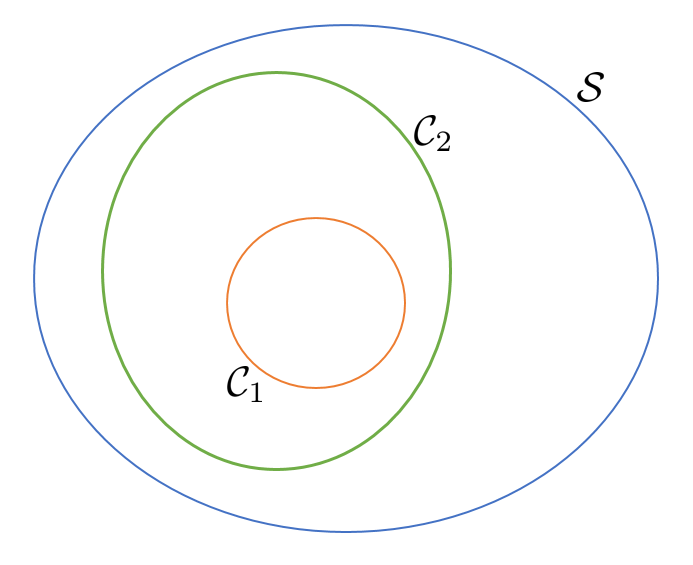
\includegraphics[width=0.5\textwidth]{f2.png}
	\caption{Example of $\mathcal{S},\mathcal{C}_1,\mathcal{C}_2$}
\end{figure}

Let $E_1$: choice is in set $\mathcal{C}_1$ when $\mathcal{S}$ is offered, $E_2$: choice is in set $\mathcal{C}_2$ when $\mathcal{S}$ is offered, $E_1 \subseteq E_2$, then
\begin{align}
\mathbb{P}(\mathcal{C}_1|\mathcal{S})&=Pr(E_1)\\
&=Pr(E_1\cap E_2)\\
&=Pr(E_1|E_2)\cdot Pr(E_2)\\
&=Pr(E_1|E_2)\cdot Pr(\mathcal{C}_2|\mathcal{S}).
\end{align}

Let $E$: choice is in set $\mathcal{C}_1$ when \underline{offered $\mathcal{C}_2$}, then
\begin{equation}
Pr(E) = \mathbb{P}(\mathcal{C}_1|\mathcal{C}_2).
\end{equation}
In other words, Luce's Axiom is imposing that
\begin{equation}
Pr(E_1|E_2)=Pr(E).
\end{equation}
Writing (12) in English is that Pr(choice in $\mathcal{C}_1$ when $\mathcal{S}$ offered $|$ choice in $\mathcal{C}_2$ when $\mathcal{S}$ offered) = Pr(choice in $\mathcal{C}_1$ when $\mathcal{C}_2$ is offered), which means that rest of items are irrelevant if knowing choice is from $\mathcal{C}_2$.

For example, $\mathcal{S}$=\{car, bike, train, bus\}, $\mathcal{C}_1=\{bus\}$, $\mathcal{C}_2=\{bus,train\}$.

Conditioned on the fact that the choice belongs to $\mathcal{C_2}$, the probability that the choice belongs to $\mathcal{C}_1$ does not depend on the larger set $\mathcal{S}$. Therefore, for the purpose of choosing from the set $\mathcal{C}_2$, the elements in the set $\mathcal{S} \setminus \mathcal{C}_2$ become \underline{irelevant}. Because of this, this property is also called the \textbf{Independent of Irrelevant Alternatives} (IIA) property.

IIA is a term that was used by Kenneth Arrow in his set of axioms. It was explained through the following example:\\
\indent Initial set: \{\underline{apple pie},blueberry pie\}\\
\indent Final set: \{apple pie, \underline{blueberry pie}, cherry pie\}
\begin{proposition}
	For any two items, $i,j\in \mathcal{S}_1,\mathcal{S}_2$, then the choice axiom implies that
	\begin{equation}
	\dfrac{\mathbb{P}(i|\mathcal{S}_1)}{\mathbb{P}(j|\mathcal{S}_1)}=\dfrac{\mathbb{P}(i|\mathcal{S}_2)}{\mathbb{P}(j|\mathcal{S}_2)}.
	\end{equation}
\end{proposition}
\begin{proof}
	Let $\mathcal{C}_1 = \{i\}$, $\mathcal{C}_2=\{i,j\}$, $\mathcal{S}=\mathcal{S}_1$. By Luce's choice axiom, we have
	\begin{equation}
	\mathbb{P}(i|\mathcal{S}_1)=\mathbb{P}(\mathcal{C}_2|\mathcal{S})\cdot \mathbb{P}(\mathcal{C}_1|\mathcal{C}_2)=\mathbb{P}(\{i,j\}|\mathcal{S}_1)\cdot \mathbb{P}(i|\{i,j\}).
	\end{equation}
	Similarly, we get
	\begin{equation}
	\mathbb{P}(j|\mathcal{S}_1)=\mathbb{P}(\{i,j\}|\mathcal{S}_1)\cdot \mathbb{P}(j|\{i,j\}).
	\end{equation}
	\begin{equation}
	\Rightarrow \dfrac{\mathbb{P}(i|\mathcal{S}_1)}{\mathbb{P}(j|\mathcal{S}_1)}=\dfrac{\mathbb{P}(\{i,j\}|\mathcal{S}_1)\cdot \mathbb{P}(i|\{i,j\})}{\mathbb{P}(\{i,j\}|\mathcal{S}_1)\cdot \mathbb{P}(j|\{i,j\})} = \dfrac{\mathbb{P}(i|\{i,j\})}{\mathbb{P}(j|\{i,j\})}.
	\end{equation}
	
	In a similar fashion, we can show that 
	\begin{equation}
	\dfrac{\mathbb{P}(i|\mathcal{S}_2)}{\mathbb{P}(j|\mathcal{S}_2)}=\dfrac{\mathbb{P}(i|\{i,j\})}{\mathbb{P}(j|\{i,j\})}.
	\end{equation}
\end{proof}

It can be shown that Luce's choice model is equivalent to the MNL model. \underline{Hint}: (Go from Luce's to MNL) Set $v_i = \mathbb{P}(i|\mathcal{N})$ \& choice axiom $\Rightarrow$ $\mathbb{P}(i|\mathcal{S})=\dfrac{v_i}{\sum\limits_{j\in \mathcal{S}}v_j}$.

\section{Red bus - Blue bus example}
Setting:
\begin{itemize}
	\item Bus, Train: People are indifferent between the two. 50\% take Bus and 50\% take Train.
	\item Bus: Split into two choices: red bus \& blue bus.	If we offer red and blue buses, then customer split evenly between the two.
\end{itemize}

Now suppose we offer all the three options: \{Red bus, Blue bus, Train\}. 25\% choose red bus, 25\% choose blue bus, and the remaining 50\% choose the train.

$\mathcal{S}=\{R,B,T\}$, $\mathcal{C}_2=\{B,T\}$, $\mathcal{C}_1=\{B\}$

Given the choice probability from offering $\mathcal{S}$, $Pr(\mathcal{C}_1|\mathcal{S})=\frac{1}{4}$, $Pr(\mathcal{C}_2|\mathcal{S})=\frac{3}{4}$. By the choice axiom, it follows that
\begin{equation}
\mathbb{P}(\mathcal{C}_1|\mathcal{C}_2)=\dfrac{\mathbb{P}(\mathcal{C}_1|\mathcal{S})}{\mathbb{P}(\mathcal{C}_2|\mathcal{S})}=\dfrac{1/4}{3/4}=\frac{1}{3}.
\end{equation} 
$\Rightarrow$ $Pr(\text{Blue bus is chosen from Blue bus \& Train})=\frac{1}{3}$.

An implication of Luce's Axiom is proportional substitution, i.e., when an option is dropped from the offer set, customer who used to buy that option substitute to other items in proportion to their corresponding market shares.

\begin{figure}[H]
	\centering
	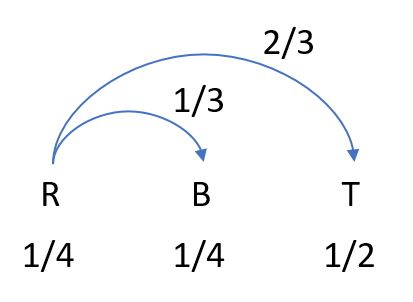
\includegraphics[width=0.5\textwidth]{f3.png}
	\caption{Substitution under Luce's Axiom}
\end{figure}

\section{Taking the MNL model to practice}
So far, we have focused on $\epsilon$ (the error term). We now focus on the deterministic component, $V$.

One of key functions of the MNL model is to understand how various factors affect choices of customers. It can be used to (a) explain choice in terms of factors affecting it; (b) run counter factuals: what would happend if price or another feature is changed; (c) allows one to put a \$ value on different attributes.

Let's assume the following:
\begin{equation}
utility = f(attributes,price).
\end{equation}

We now express the deterministic component of the utility in terms of \underline{observable} features. We distinguish two types of features: (a) alternative-specific: price, color, packaging, flavors; (b) individual/choice instance specific: income, gender, time of day, geographic location, etc.

We typically express this as
\begin{equation}
V_{ij}=f(\underline{z}_{ij},\underline{s}_i),
\end{equation} 
where 
\begin{itemize}
	\item $V_{ij}$: Deterministic utility for item $j$ in choice instance $i$.
	\item $\underline{z}_{ij}$: Vector of alternative specific attributes.
	\item $\underline{s}_i$: Vector of individual/choice instance specific attributes.
\end{itemize}

We use the standard assumption that $f(\cdot,\cdot)$ is \underline{linear-in-parameters}. In other words, $f(\cdot,\cdot)$ must be linear in the parameters that describe the model and not necessarily linear in attributes. 

\begin{equation}
V_{ij} = \underline{\beta}^\intercal \begin{bmatrix}
\underline{z}_{ij}\\
\underline{s}_i
\end{bmatrix},
\end{equation}
where $\underline{\beta}$ are parameters and $\begin{bmatrix}
\underline{z}_{ij}\\
\underline{s}_i
\end{bmatrix}$ are attributes.

We distinguish two types of coefficients:
\begin{enumerate}
	\item[(a)] generic coefficients: coefficients that stay the same across the alternatives.
	\item[(b)] alternative specific coefficients: coefficients specific to each alternative.
\end{enumerate}

Therefore, we can write (21) into the following form,
\begin{equation}
V_{ij} = \alpha_j + \underline{\beta}^\intercal \underline{z}_{ij} + \underline{\gamma}_j^\intercal \underline{s}_i + \underline{\delta}_j^\intercal \underline{w}_{ij},
\end{equation}
where
\begin{itemize}
	\item $\alpha_j$: intercept term/ Alternative Specific Constant (ASC).
	\item $\underline{\beta}$: generic coefficients (does \underline{not} depend on $j$).
	\item $\underline{\beta}^\intercal \underline{z}_{ij}$: generic coefficients - alternative specific attributes ($\beta\times Price_{ij}$).
	\item $\underline{\gamma}_j$: alternative specific coefficients (depend on $j$).
	\item $\underline{\gamma}_j^\intercal \underline{s}_i$: alternative specific coefficients - individual specific attributes ($\gamma_j \times Income_i$).
	\item $\underline{\delta}_j$: alternative specific coefficients.
	\item $\underline{\delta}_j^\intercal \underline{w}_{ij}$: alternative specific coefficients - alternative specific attributes ($\delta_j\times Price_{ij}$).
\end{itemize}
\end{document}
